\section{Defining Community Core}

Previous attempts for identifying the community core of a scientific community are based on algorithmic approaches that aim at identifying dense clusters of nodes in the
network~\cite{Seifi:2012:CCE:2187980.2188258}.  However, as we plan to investigate the role of a core in the network structure, any approach that makes use of the network structure
to identify such nodes could lead us to a biased set of authors. Instead, we focus on developing a metric that quantifies the involvement of a researcher in a scientific community
during a certain period of time.  Intuitively, this metric should be able to capture i) the prolificness of an author in different communities and ii) the frequency of involvement
of the author with the community in a certain period of time.

First, in order to capture the prolificness of an author, we use a common metric namely h-index~\cite{Hirsch:2005}. This metric consists of an index that attempts to measure both
the productivity and impact of the published work of a researcher. It is based on the set of the researcher's most cited papers and the number of citations that they have received.
More specifically, a researcher $a$ has h-index $h_a$ if $h$ of her N papers have at least h citations each, and the other (N − h) papers have no more than h citations each. Thus,
if an author have 10 papers with at least 10 citations, she has h-index 10.  

Second, as an attempt to capture the importance of an author to a specific community in a certain period of time, we multiple the h-index by the number of publications this author
has in a certain community during a time window. We name this measure as \textit{Core Score}. More formally, the Core Score of an author $a$ in a community $c$ during a period of
time $t$, $Core{ }Score_{a,c,t}$, is given by its $h\textrm{-}index_a$ multiplied by the number of publications $a$ has in $c$ during $t$.

\begin{equation} 
  \label{eq:core_score}
  Core{ }Score_{a,c,t} = h\textrm{-}index_a * number\textrm{ }of\textrm{ }publications_{a,c,t}
\end{equation}

We note that the first part of the equation captures the importance of an author to the scientific community in different areas and periods and the second part weight this
importance based on the activity of the author in a certain community and time.  By computing the core score for the members of a community we define the community core in a
certain period of time as the top researchers of that community in terms of their core scores in the given period. Next, we detail how we inferred the h-index of authors in
Section~\ref{sub:hindex}.  Then, Section~\ref{sub:thresholds} discusses how we define two important thresholds: the size of the community core and the time window used in our
analyses.


\subsection{Inferring Authors H-index}
\label{sub:hindex}

There are multiple tools that measure the h-index of research authors, out of which Google Citations\footnote{http://scholar.google.com/citations} is the most prominent one.
However, to have a profile in this system, a researcher needs to sign up and explicitly create her research profile.  In a preliminary data collection of part of the profiles of
the DBLP authors we found that less than 30\% of the authors of these communities had a profile in the Google citations. Thus, this strategy would reduce our dataset and
potentially introduce bias for network analysis.
 
To divert from this limitation, we used data from SHINE, the Simple HINdex Estimation project\footnote{http://shine.icomp.ufam.edu.br/}, to infer community authors' h-index  .
SHINE is a search system that allows users to check the h-index of thousands of computer science conferences. They crawled google scholar, searching for the title of papers
published in a number of conferences, which allowed them to effectively estimate the h-index of these target conferences based on the citations computed by google scholar. Although
SHINE does not allow one to search for an author instead of a conference, the shine builders kindly allowed us to access their database to infer the h-index of authors based on the
conferences they crawled.


\begin{figure}[!htb]
\centering
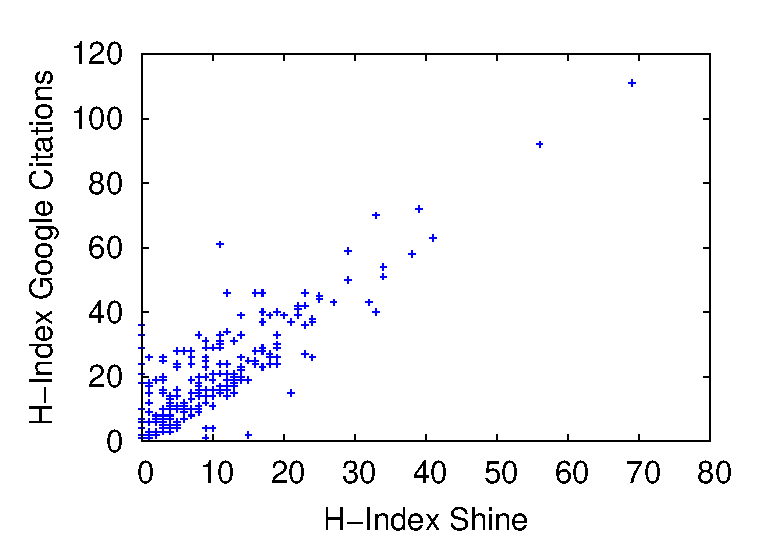
\includegraphics[scale=.5]{graficos/hindex/hindex_scatter_plot.eps}
\caption{Correlation between the inferred H-Index and Google Scholar Citations }
\label{fig:hindex_scatter_plot}
\end{figure}


There is one important limitation with this strategy.  As SHINE does not track all the existent computer science conferences, authors' h-index might be underestimated when computed
with this data. To investigate this issue, we compared the h-index of a set of authors with account on Google citations with their estimated h-index based on the SHINE dataset.  We
randomly selected 10 researchers for each conference from Table~\ref{tab:sigs_conference_period} and we extracted their h-index from their Google scholar profiles.  In comparison
with the H-index we estimated from SHINE, the Google scholar values are, in average, 50\% higher. Figure~\ref{fig:hindex_scatter_plot} shows the scatter plot for the two h-index
measures. We can note that although SHINE h-index is smaller, the two measures are highly correlated. The pearson correlation coefficient is 0.85, which indicates that authors
might have proportional h-index estimations in the two systems. 

\subsection{Setting the thresholds}
\label{sub:thresholds}


There are two important thresholds in our approach we need to define to determine the core of a scientific community.  The first is related to the time window in which the core
community is computed. In other words, should we compute the community core at each year, at each two years, or for a larger time window? The second threshold is related to the
size of the community core. As we define the core of a community as the top researchers in terms of their core score during a certain time window, it is important to define the
threshold for choosing the top ones.

Our strategy to define these thresholds consists of varying each of them and quantifying how they impact on the changes on the members of the community core. To measure these
changes, we compute a metric namely resemblance, as used in~\cite{Viswanath:2009}, which measures the fraction of members in the core at time $t_0$ and remain in the core at the
time $t_1$. For each conference, we vary the window size from 1 to 5 years and the size of community core from 10\% to 60\% of the entire community.

Intuitively, high resemblance variations indicate bad threshold choices, and thus, we should seek for values in which threshold changes causes slightly changes on resemblance.
Figure~\ref{fig:averange_values_resemblance} shows the resemblance values as a function of the window size, providing different curves for the community core size.  We choose the
SIGMOD and CHI for this analysis. The rest of the communities are omitted due to lack of space, but the same observations hold for them. By visual inspection we would set the core
size as 10\% due to the proximity of the curves and the window size as 2 or 3, as most of the communities showed a more stable resemblance after these values. To help us decide we
compute the angular coefficient for the 10\% core size curves of each community and obtained the average angular coefficient for them.  Based on this value, we choose the window
size for our experiments as 3.

\begin{figure}[!htb]
  \begin{center}
    \subfigure[SIGMOD]{%
      \label{fig:sigmod_slide_window_top_list}
      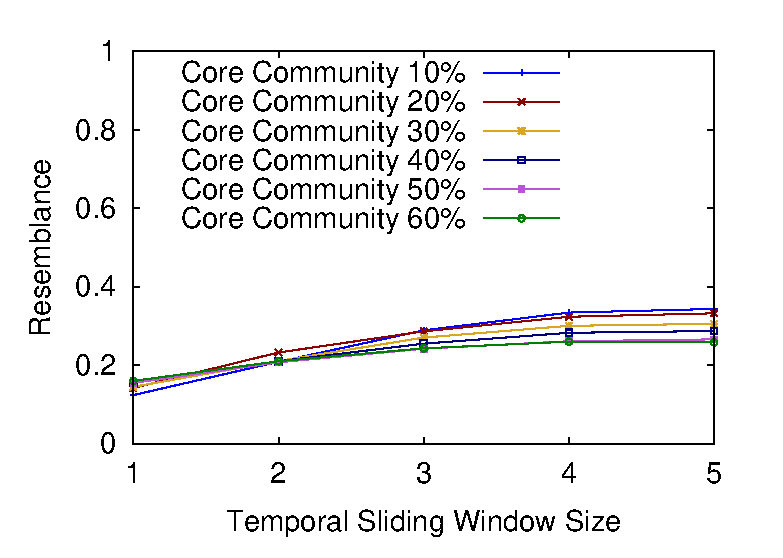
\includegraphics[scale=.33]{graficos/window_core_size/sigmod_slide_window_top_list.eps}
    }%
    \subfigure[CHI]{%
      \label{fig:chi_slide_window_top_list}
      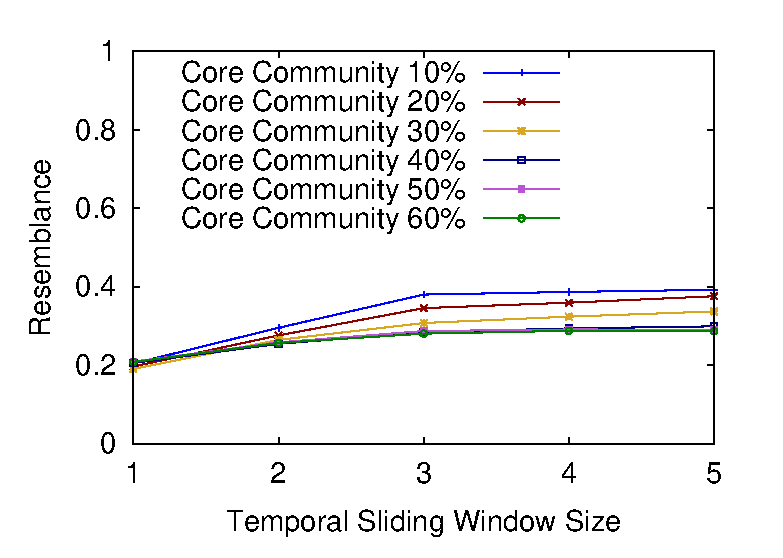
\includegraphics[scale=.33]{graficos/window_core_size/chi_slide_window_top_list.eps}
    }%
  \end{center}
\caption{Average of the values of resemblance}
 \label{fig:averange_values_resemblance}
\end{figure}


\subsection{Validation}

Based on the measure of core score, we expect that the members of the community core would be members of standing that actively contribute with publications to a certain community.
The validation of these matters is, by nature, subjective.  Next, we provide evidences that our approach correctly captures these expected properties.

First, we analyze the core score of two WWW 2013 keynote speackers: Jon Kleinberg and Luis von Ahn.  Figure~\ref{fig:rank_core_score_authors} shows the ranking position in terms of
percentage (i.e. position 5\% of that community) of these two authors in the communities they have published. The red line divides the members of the community core from the other
members. We can note that Jon Kleinberg was a member of the community core of STOC for years, a theoretical conference. Indeed, he was part of the STOC core for \red{twelve} years,
publishing seven STOC papers in a single period of three years. With Kleinberg's involvements on KDD, he became less active in STOC and left the core that community for some time.
During this period he published several KDD papers, whereas his publications in STOC were drastically reduced.  When it comes to Luis von Ahn, we can note that he is more active in
the CHI community, a community in which he published 6 papers along his academic life. He reached the core of the CHI community along three consecutive time windows,
publishing four CHI papers in a single period.



\begin{figure}[!htb]
  \begin{center}
    \subfigure[Jon Kleinberg]{%
      \label{fig:cc_kleinberg}
      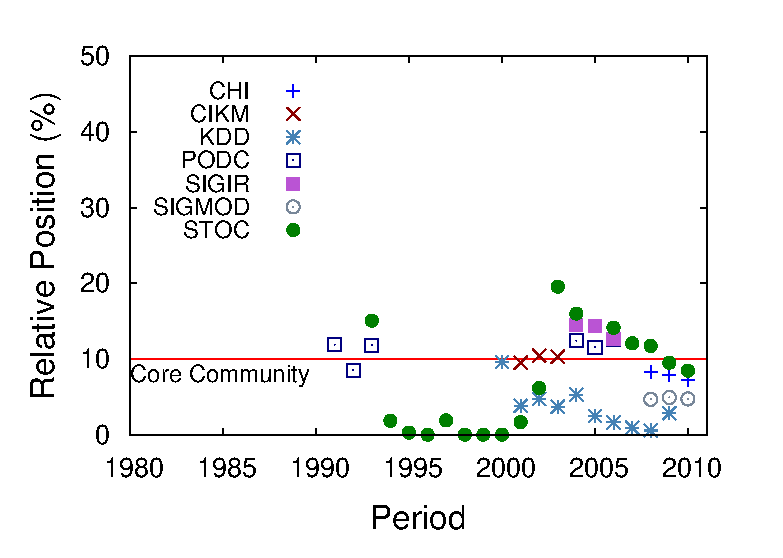
\includegraphics[scale=.33]{graficos/validacao_core_community/cc_kleinberg.eps}
    }%
    \subfigure[Luis von Ahn]{%
      \label{fig:cc_luis_von_ahn}
      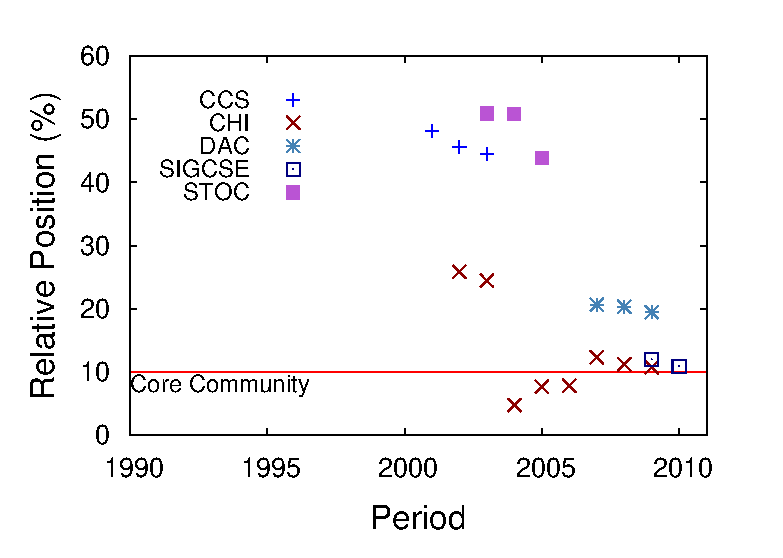
\includegraphics[scale=.33]{graficos/validacao_core_community/cc_luis_von_ahn.eps}
    }%
  \end{center}
\caption{Core score of two WWW 2013 keynote speakers}
 \label{fig:rank_core_score_authors}
\end{figure}


Next, we compute a ranking of researchers that appear most often in the community core of each scientific community.  We choose the CIKM, KDD, SIGIR, and SIGMOD to show the
top 20 researchers in Table~\ref{tab:authors_frequency_core_community} as they are Web related conferences.  
We can note that several big names appear in this ranking, including past keynote speakers of these events
as well as awarded authors by their life time contributions in that community. Indeed, by analyzing the awarded researchers
from SIGMOD and SIGIR we found that a large fraction of them appeared in the community core at least one time in the conference history. More specifically, these fractions
are 60\% of the awarded SIGIR\footnote{http://www.sigir.org/awards/awards.html} members and 80\% for SIGMOD\footnote{http://www.sigmod.org/sigmod-awards}. These observations
provides evidences that our approach correctly captures the notion of a scientific community core.

\begin{table*}[!htb]
\centering
\caption{Researchers who appear most often in the Core Community over the years.}
\label{tab:authors_frequency_core_community}
{\small
\begin{tabular}{|c|l|l|l|l|} \hline
 & \bf CIKM & \bf KDD &\bf  SIGIR & \bf SIGMOD\\ \hline
1\textsuperscript{st} & Philip S. Yu & Heikki Mannila & W. Bruce Croft* & David J. DeWitt*\\ \hline
2\textsuperscript{nd} & Jiawei Han & Jiawei Han & Clement T. Yu & Michael Stonebraker*\\ \hline
3\textsuperscript{rd} & Ling Liu & Eamonn J. Keogh & Susan T. Dumais* & H. V. Jagadish\\ \hline
4\textsuperscript{th} & Clement T. Yu & Martin Ester & James Allan & Rakesh Agrawal*\\ \hline
5\textsuperscript{th} & Christos Faloutsos & Bing Liu & Justin Zobel & Christos Faloutsos\\ \hline
6\textsuperscript{th} & James Allan & Padhraic Smyth & Alistair Moffat & Raghu Ramakrishnan\\ \hline
7\textsuperscript{th} & Elke A. Rundensteiner & Charu C. Aggarwal & Norbert Fuhr* & Jiawei Han\\ \hline
8\textsuperscript{th} & Ke Wang & Philip S. Yu & James P. Callan & Gerhard Weikum\\ \hline
9\textsuperscript{th} & Amr El Abbadi & Ke Wang & Yiming Yang & Philip A. Bernstein*\\ \hline
10\textsuperscript{th} & W. Bruce Croft & Hans-Peter Kriegel & Edward A. Fox & Jeffrey F. Naughton\\ \hline
11\textsuperscript{th} & Ming-Syan Chen & Rakesh Agrawal & Gerard Salton* & Hector Garcia-Molina*\\ \hline
12\textsuperscript{th} & Divyakant Agrawal & Jian Pei & Ricardo A. Baeza-Yates & Michael J. Carey*\\ \hline
13\textsuperscript{th} & C. Lee Giles & Wynne Hsu & Jian-Yun Nie & Joseph M. Hellerstein\\ \hline
14\textsuperscript{th} & Weiyi Meng & Qiang Yang & Mark Sanderson & Philip S. Yu\\ \hline
15\textsuperscript{th} & Berthier A. Ribeiro-Neto & Christos Faloutsos & Charles L. A. Clarke & Divesh Srivastava\\ \hline
16\textsuperscript{th} & M. Tamer \"Ozsu & Huan Liu & Chris Buckley & Michael J. Franklin\\ \hline
17\textsuperscript{th} & ChengXiang Zhai & Mohammed Javeed Zaki & ChengXiang Zhai & Jennifer Widom*\\ \hline
18\textsuperscript{th} & Javed A. Aslam & Pedro Domingos & Alan F. Smeaton & Hans-Peter Kriegel\\ \hline
19\textsuperscript{th} & Hans-Peter Kriegel & Jon M. Kleinberg & Zheng Chen & Hamid Pirahesh\\ \hline
20\textsuperscript{th} & Bing Liu & Vipin Kumar & Ophir Frieder & Surajit Chaudhuri*\\ \hline
\end{tabular}
}
\par\medskip\footnotesize{* Researchers awarded by a lifetime of innovation and leadership inside that community.}
\end{table*}

%   & \bf{CHI} & \bf{SIGCOMM} & \bf{SIGIR} & \bf{SIGMOD}\\ \hline
% 1\textsuperscript{st} & Scott E. Hudson & Scott Shenker & W. Bruce Croft & David J. DeWitt\\ \hline
% 2\textsuperscript{nd} & Elizabeth D. Mynatt & George Varghese & Clement T. Yu & Michael Stonebraker\\ \hline
% 3\textsuperscript{rd} & Hiroshi Ishii & Hui Zhang & Susan T. Dumais & H. V. Jagadish\\ \hline
% 4\textsuperscript{th} & Steve Benford & Donald F. Towsley & James Allan & Rakesh Agrawal\\ \hline
% 5\textsuperscript{th} & Shumin Zhai & Hari Balakrishnan & Justin Zobel & Christos Faloutsos\\ \hline
% 6\textsuperscript{th} & Brad A. Myers & Ion Stoica & Alistair Moffat & Raghu Ramakrishnan\\ \hline
% 7\textsuperscript{th} & Ravin Balakrishnan & Srinivasan Seshan & Norbert Fuhr & Jiawei Han\\ \hline
% 8\textsuperscript{th} & James A. Landay & Deborah Estrin & James P. Callan & Gerhard Weikum\\ \hline
% 9\textsuperscript{th} & George G. Robertson & David Wetherall & Yiming Yang & Philip A. Bernstein\\ \hline
% 10\textsuperscript{th} & Michael J. Muller & Thomas E. Anderson & Edward A. Fox & Jeffrey F. Naughton\\ \hline
% 11\textsuperscript{th} & Mary Czerwinski & Jennifer Rexford & Gerard Salton & Hector Garcia-Molina\\ \hline
% 12\textsuperscript{th} & Robert E. Kraut & Jia Wang & Ricardo A. Baeza-Yates & Michael J. Carey\\ \hline
% 13\textsuperscript{th} & Loren G. Terveen & Ratul Mahajan & Jian-Yun Nie & Joseph M. Hellerstein\\ \hline
% 14\textsuperscript{th} & Carl Gutwin & Vern Paxson & Mark Sanderson & Philip S. Yu\\ \hline
% 15\textsuperscript{th} & Ken Hinckley & Mark Handley & Charles L. A. Clarke & Divesh Srivastava\\ \hline
% 16\textsuperscript{th} & W. Keith Edwards & Yin Zhang & Chris Buckley & Michael J. Franklin\\ \hline
% 17\textsuperscript{th} & Gregory D. Abowd & Peter Steenkiste & Chengxiang Zhai & Jennifer Widom\\ \hline
% 18\textsuperscript{th} & Anind K. Dey & Walter Willinger & Alan F. Smeaton & Hans-Peter Kriegel\\ \hline
% 19\textsuperscript{th} & Saul Greenberg & Ramesh Govindan & Zheng Chen & Hamid Pirahesh\\ \hline
% 20\textsuperscript{th} & Susan T. Dumais & Jon Crowcroft & Ophir Frieder & Surajit Chaudhuri\\ \hline

